\section{Cell Merge Performance}
In order to compare the error of the proposed cell merge with that of the Voronoi tessellation, a set of 1000 unique sources was randomly generated. Using these sources, 1000 tessellations were generated using each algorithm yielding 1 to 1000 cells per generation. For the Voronoi, the brightest sources were chosen as centres for the tessellation in each iteration. The Voronoi structures were re-centred to minimise the error as much as possible. For each iteration of the cell merge algorithm, the space was tessellated using all 1000 sources as centres and the merge process was iterated until the desired number of cells was reached. For each iteration of both algorithms, the total error for the space was calculated and stored.
\\
\\
While both algorithms place their centres optimally within their cells, the structure of the cells generated in the cell merge are dependent on the intensities and positions of all sources in the space while those in the Voronoi are generated in a way that is dependent only on the positions of the sources with the highest intensities. Figure \ref{res:fig:error} shows the error for a set number of cells for a fixed set of sources while Figure \ref{res:fig:error_log} shows the logarithmic scaled version of the resulting error data.
\\
\\
As shown, both algorithms have zero error when generating 1000 cells but once the number of cells decreases, the error begins to increase exponentially. Figure \ref{res:fig:error} therefore shows that the cell merge algorithm has a lower error compared with that of the Voronoi algorithm for a high number of centres. Figure \ref{res:fig:error_log_z} shows that for a very small number of cells, the Voronoi tessellation is more feasible. While both still have extremely large errors, the error of the Voronoi is lower than that of the cell merge algorithm until they once again meet when a single cell is used to generate the Voronoi.
\begin{figure}[H]
\centering
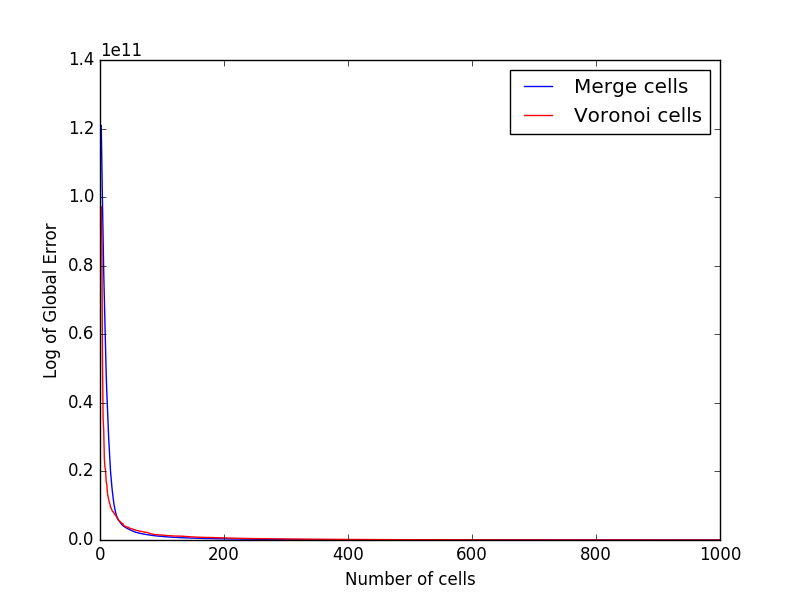
\includegraphics[width=0.8\textwidth]{Images/result_error.png}
\caption{A comparison of the total error of the Voronoi tessellation (red) and the cell merge (blue) algorithms.}
\label{res:fig:error}
\end{figure}
\begin{figure}[H]
\centering
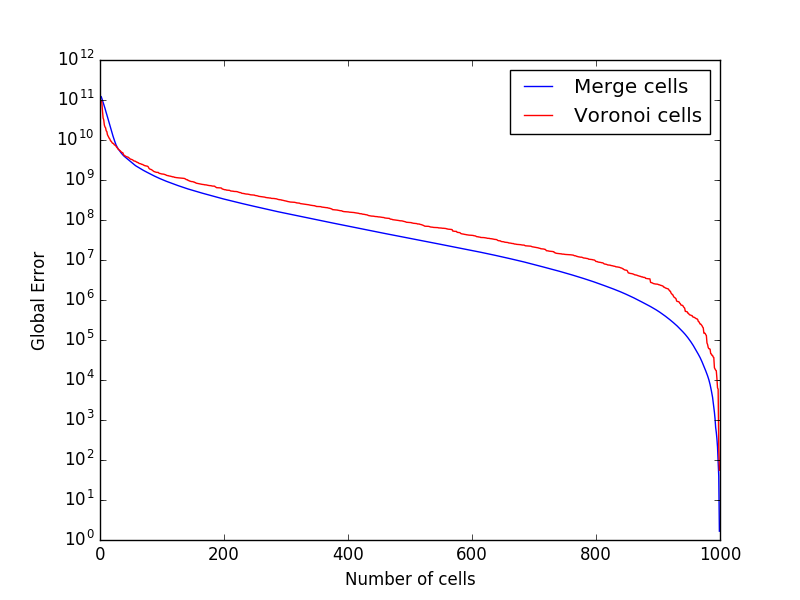
\includegraphics[width=0.7\textwidth]{Images/result_error_log.png}
\caption{A logarithmic scale of the data presented in Figure \ref{res:fig:error}.}
\label{res:fig:error_log}
\end{figure}
\begin{figure}[H]
\centering
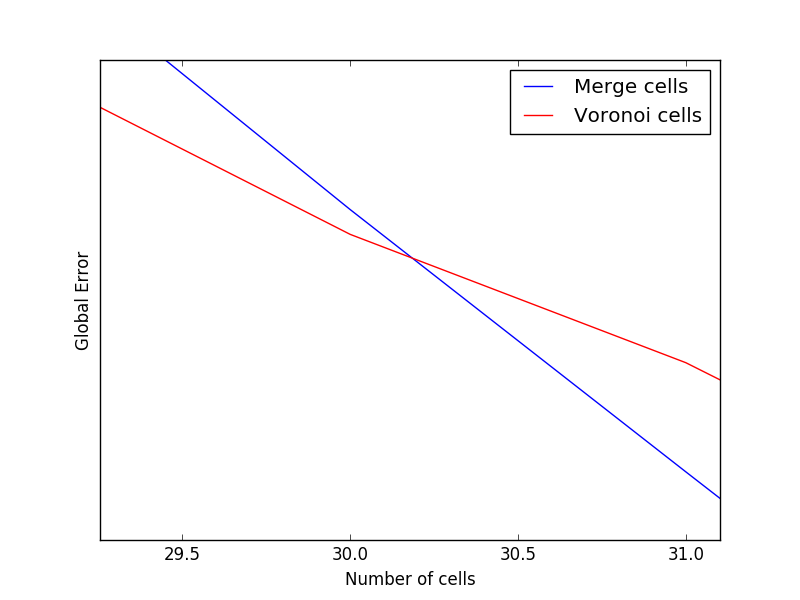
\includegraphics[width=0.8\textwidth]{Images/result_error_log_zoom.png}
\caption{A close up of the logarithmic scale data showing the point at which the cell merge and Voronoi intercept.}
\label{res:fig:error_log_z}
\end{figure}